\section{Resultados e Discussão}\label{sec-resultados}

Considerando as particularidades de ensinar para o público adulto, que
grande parte das vezes consorcia o aprendizado com a rotina de trabalho,
as TDIC podem ser uma excelente alternativa para não apenas promover uma
aprendizagem mais significativa, mas também desenvolver a fluência
tecnológica, característica essa tão necessária no mundo do trabalho
atualmente. Nessa perspectiva buscou-se compreender como essa temática
vem sendo estudada nos programas de pós-graduação brasileiros, por meio
da análise cienciométrica.

Dos trabalhos retornantes (15+4), 5 deles eram repetidos. Os demais
trabalhos descartados, possuíam apenas algum dos descritores de forma
aleatória ao longo do texto, mas não tinham esse foco de pesquisa. O
baixo número de trabalhos retornantes está alinhado aos dados reportados
na literatura por \textcite{BrancoPinto2022}. Neste sentido, foram analisados
9 trabalhos, sendo os dados da análise apresentados a seguir.
Inicialmente, buscamos compreender como as produções estavam
distribuídas temporalmente (\Cref{fig2}).

\begin{figure}[!htpb]
\centering
\begin{minipage}{.5\textwidth}
\caption{Distribuição das produções por ano e tipo.}\label{fig2}
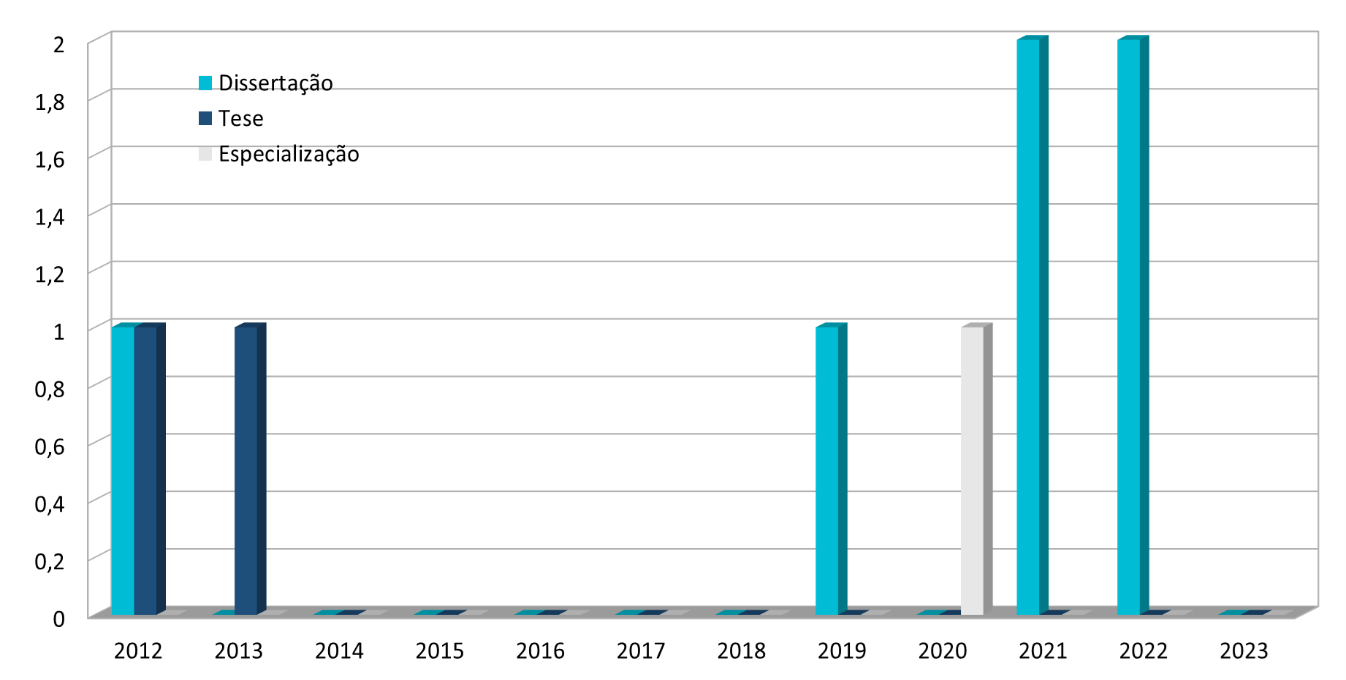
\includegraphics[width=\textwidth]{Fig2.png}
\source{as autoras.}
\end{minipage}
\end{figure}


Como pode-se observar na \Cref{fig2}, as produções são aleatoriamente
distribuídas ao longo destas duas décadas, sendo os anos de 2012 e 2021,
os que apresentam maior número de produção. Este fato pode estar
correlacionado com as políticas públicas de incentivo à Educação
Profissional, com a criação dos Institutos Federais. Observa-se ainda
uma lacuna de produção entre os anos de 2013 e 2018. Estes dados são
discordantes dos encontrados por \textcite{vieira2021}, que ao
estudarem a produção sobre PROEJA na plataforma Web of Science,
encontraram 33 documentos, sendo 27\% destes publicados no ano de 2016.

Em relação a modalidade da produção, pode-se verificar conforme os dados
da \Cref{fig2}, que a maioria da produção refere-se a dissertações de
mestrado (6 produções -- 66,7\%), seguido das teses (2 produções --
22,2\%) e apenas uma monografia de especialização (11,1\%). Estes dados
são concordantes com os encontrados por \textcite{minuzzi2020}, que
analisaram a produção do conhecimento do Ensino Médio integrado a EPT.
Segundo os autores, esse dado pode ser compreendido pelo tempo de
pesquisa envolvido no mestrado (24 meses), quando comparado ao de
doutorado (48 meses). No entanto, o mesmo não aponta para nenhuma
monografia na área.

Com a intenção de compreender a distribuição da produção sobre
tecnologias digitais imbricadas com a educação profissional de jovens e
adultos, analisou-se como estas encontram-se distribuídas por regiões,
sendo os dados apresentados na \Cref{fig3}. Como pode-se observar na
Figura, as regiões sul e nordeste são as que mais contribuíram para a
produção do conhecimento nesta área, contradizendo os achados de \textcite{barros_producao_2019}, que ao analisar a produção apresentada na Associação Nacional de Pós-Graduação em Educação (ANPEd), no interstício de 2007 a 2017, apontam a região sudeste como a maior produtora de conhecimento.

\begin{figure}[!htpb]
\centering
\begin{minipage}{.5\textwidth} 
\caption{Distribuição das produções pelas regiões do Brasil.}\label{fig3}
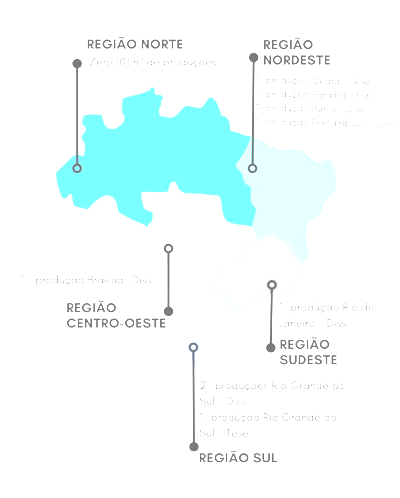
\includegraphics[width=\textwidth]{Fig3.png}
\source{as autoras}
\end{minipage}
\end{figure}

Os dados levantados nesta pesquisa, que apontam as regiões sul e
nordeste como maiores produtores de saberes, poderiam estar relacionados
ao fato de termos tanto no Rio Grande do Norte (PPGEP), como no Rio
Grande do Sul (PPGEPT), programas de pós-graduação em Educação
Profissional e Tecnológica, os quais têm como objeto de estudo todas as
modalidades da EPT, além do Programa em Rede em Educação Profissional e
Tecnológica, que abrange diversas instituições de Ensino superior
Federal do Brasil (ProfEPT). No entanto, analisando os dados retornantes
da busca, pode-se verificar que tanto o PPGEPT, como o ProfEPT,
apresentam cada um apenas uma produção, enquanto o PPGEP nenhuma, o que
não corrobora com essa hipótese. No intuito de verificar se as produções encontradas eram referentes a estes programas, mapeou-se a distribuição de teses e dissertações por programa, instituição de ensino e tipo de programa (acadêmico ou profissional). Os dados retornantes da análise podem ser visualizados na \Cref{tab-01}.

\begin{table}
\centering
\begin{threeparttable}
\caption{Distribuição de teses e dissertações por programa.}\label{tab-01}
\begin{tabular}{lllll}
\toprule
Programa & Nº de produções & Instituição & Área do Programa & Tipo\\
\midrule
PPGE & 1 & UFC & Educação & Acadêmico \\
PPGCLIP & 1 & UFBA & Educação & Profissional \\
\multicolumn{1}{p{4cm}}{\small Especialização em Línguas Estrangeiras Modernas} & 1 & IFPB & \textemdash & --- \\
PPGEPT & 1 & UFSM & Interdisciplinar & Acadêmico \\
PPGIE & 1 & UFRGS & Interdisciplinar & Acadêmico \\
PPGEnsino & 1 & UNIVATES & Ensino & Acadêmico \\
PPGEA & 1 & UFRRJ & Educação & Profissional \\
MNPEF & 1 & UnB & Astronomia / Física & Profissional \\
ProfEPT & 1 & IFPE & Ensino & Profissional \\
\bottomrule
\end{tabular}
\source{as autoras.}
\end{threeparttable}
\end{table}


Ao analisar a \Cref{tab-01}, verifica-se três produções em programas da área
de educação, sendo dois profissionais e um acadêmico, assim como dois da
área interdisciplinar, dois na área de ensino e um na área de
física/astronomia. Destas produções, apenas duas são pertencentes a
programas que tem como foco da pesquisa a Educação Profissional: uma do
PPGEPT (Programa de pós-graduação em Educação Profissional e
Tecnológica) e outra do ProfEPT (Mestrado Profissional em Educação
Profissional e Tecnológica em Rede Nacional). Neste sentido, pode-se
inferir que o maior número de trabalhos nas regiões sul e nordeste não
possui correlação direta com os programas da área.

Outro ponto importante a partir da análise da \Cref{tab-01}, é que as
produções são de programas diferentes, o que não demonstra uma linha de
pesquisa de um autor ou grupo de pesquisa. Pode-se observar também, que
há um equilíbrio entre os programas acadêmicos e profissionais, sendo
ligeiramente superior os de cunho acadêmico e que apenas um trabalho foi
produzido em nível de especialização. Estes dados, por si só, já denotam
a importância de investigar de forma mais contundente o uso das TDIC no
âmbito do PROEJA.

No intuito de compreender quem são os pesquisadores que estudam as
tecnologias digitais no contexto do PROEJA, categorizou-se os mesmos
quanto ao gênero. Os dados obtidos podem ser visualizados na \Cref{fig4}.

\begin{figure}[!htpb]
\centering
\begin{minipage}{.5\textwidth}
\caption{Distribuição das produções quanto ao gênero do autor.}\label{fig4}
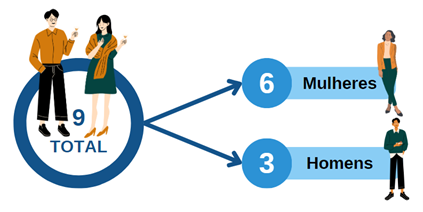
\includegraphics[width=\textwidth]{Fig4.png}
\source{as autoras.}
\end{minipage}
\end{figure}

Como pode-se observar na \Cref{fig4}, a maioria dos autores é constituída
por mulheres (66,7\%), o que pode estar relacionado com a inserção
crescente das mulheres no mundo do trabalho. Embora o número de
trabalhos retornantes neste estudo seja pequeno, pode-se inferir que a
produção de ciência pelo público feminino vem, em algumas áreas do
saber, superando o público tradicionalmente formado por homens, sendo
este dado concordante com os apontados por outros pesquisadores como
\textcite{velho2003,Leta2003,Grossi2016}. Os
autores mencionados afirmam que o crescimento do público feminino nas
Universidades em curso de graduação e pós-graduação se dá em virtude do
aumento significativo de mulheres na pesquisa.

Conhecendo a dispersão dos trabalhos por ano, regionalidade, programas e
instituições de ensino e gênero, analisaremos a partir daqui, como as
produções retornantes são distribuídas quanto ao tipo de pesquisa,
instrumentos de coleta e de análise de dados. 

A frequência dos dados analisados em relação ao tipo de pesquisa podem
ser observada na \Cref{fig5}.

\begin{figure}[!htpb]
\centering
\begin{minipage}{.5\textwidth}
\caption{Distribuição das produções quanto ao tipo de pesquisa.}\label{fig5}
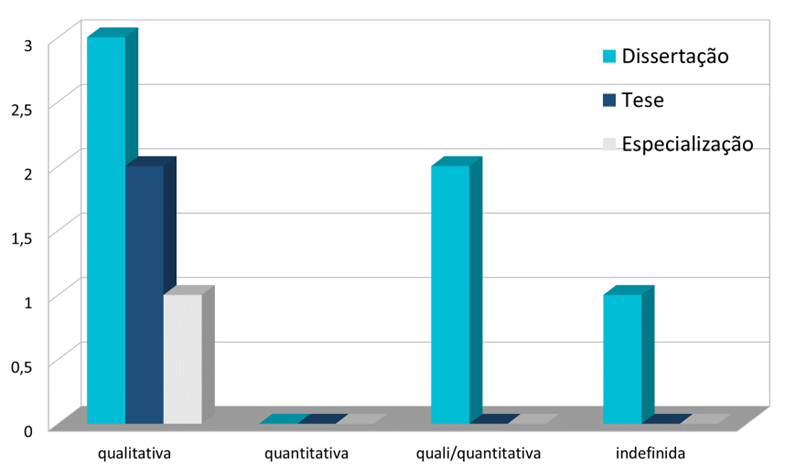
\includegraphics[width=\textwidth]{Fig5.png}
\source{as autoras.}
\end{minipage}
\end{figure}

Como é possível observar na \Cref{fig5}, quanto à abordagem, a maioria dos
trabalhos encontrados nesta busca (62,5\%) caracterizam-se por serem de
cunho qualitativo, seguido de dois trabalhos de abordagem
quali-quantitativa (25\%). Estes dados são concordantes com os
encontrados por outros pesquisadores como \textcite{minuzzi2020}, os
quais apontam em seu estudo que a pesquisa quali-quanti vem crescendo
nos últimos tempos no intuito de compreender e responder as
complexidades dos fenômenos em educação. Um dos trabalhos analisados não
apresentava clareza quanto ao tipo de abordagem utilizada, sendo
classificado como indefinido.

A preferência pelos estudos de natureza qualitativa pode estar associada
ao fato de ao menos 50\% dos trabalhos serem de programas da área de
Ensino e Educação, áreas estas que possuem tradição na análise de dados
qualitativa, como afirma \textcite{Teixeira_2015}. \textcite[p. 24]{Minayo2007}, destaca
ainda, que a pesquisa qualitativa ``[...] trabalha com o universo
dos significados, dos motivos, das aspirações, das crenças, dos valores
e das atitudes'' e, a partir desse conjunto de fenômenos humanos gerados
socialmente, busca compreender e interpretar a realidade, o que é comum
nos estudos nas áreas de ensino e de educação. Pode-se verificar ainda
na \Cref{fig5} que nenhum das produções analisadas teve foco de análise
meramente quantitativo, o que vai na mesma linha da análise feita por
\textcite{Teixeira_2015}.

Dando continuidade à análise dos trabalhos, investigou-se quais os
instrumentos de coleta de dados foram utilizados, sendo os dados
apresentados na \Cref{tab-02}.

\begin{table}
\centering
\begin{threeparttable}
\caption{Distribuição das teses e dissertações quando ao instrumento utilizado para coleta de dados.}\label{tab-02}
\begin{tabular}{llll}
\toprule
Instrumento de coleta & Tese & Dissertação & Especialização\\
\midrule		
Atividade de estudo & 0 & 1 & 0 \\
Entrevista & 2 & 2 & 0 \\
Parecer técnico & 0 & 1 & 0 \\
Questionário & 1 & 2 & 1 \\
Registro audiovisual & 0 & 1 & 0 \\
\bottomrule		
\end{tabular}
\source{as autoras.}
\end{threeparttable}
\end{table}

Como pode-se observar na \Cref{tab-02}, o principal instrumento de coleta de
dados utilizado foi a entrevista (44,4\%), sendo o instrumento adotado
em duas teses e duas dissertações. Este dado é concordante com o
esperado, visto que a maioria dos trabalhos analisados tem abordagem
qualitativa. \textcite[p.~1417]{BrancoPinto2022} mencionam que a abordagem
qualitativa ``preocupa-se com a realidade social do ser humano, se
dedica a investigar significados, motivos, valores e atitudes'', o que
pode explicar a escolha dessa.

Os questionários foram utilizados em quatro trabalhos (44,4\%), um em
nível de doutorado (que também utilizou-se de entrevista), dois de
mestrado, sendo que um deles mesclou este instrumento de coleta com a
entrevista e outro de especialização, e os demais trabalhos apresentaram
instrumentos diversos, como o registro audiovisual, parecer técnico e o
próprio uso do material didático. \textcite{minuzzi2020}, citam em
seu trabalho que após os múltiplos registros, a coleta de dados por meio
de questionários e entrevistas foram as mais encontradas.

Aqui, cabe salientar que a coleta de dados é fortemente do tipo de
pesquisa proposta e se a abordagem da mesma é do tipo qualitativa ou
quantitativa \cite{Strauss2008}. Assim, entrevistas são comumente
associadas aos trabalhos de natureza qualitativa, enquanto os
questionários permitem tanto a abordagem quali, como quantitativa. Para
compreender como os dados desses trabalhos foram analisados, os
categorizamos em descritiva, de conteúdo ou indefinida, sendo os
resultados ilustrados na \Cref{fig6}.

\begin{figure}[!htpb]
\centering
\begin{minipage}{.5\textwidth}
\caption{Distribuição das produções quanto ao tipo de análise.}\label{fig6}
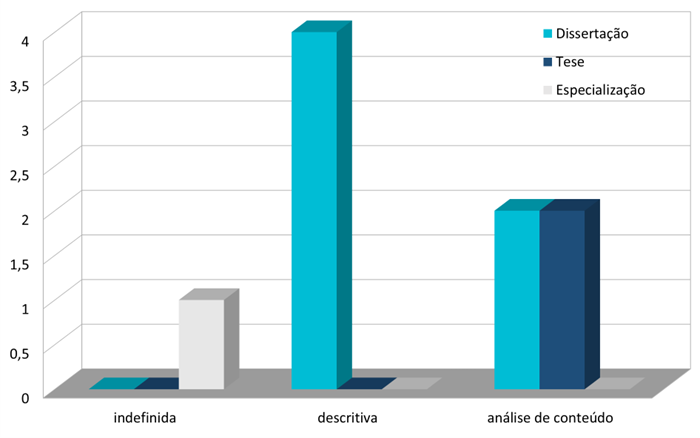
\includegraphics[width=\textwidth]{Fig6.png}
\source{as autoras.}
\end{minipage}
\end{figure}

Ao analisar a \Cref{fig6}, pode-se verificar que quatro trabalhos
utilizaram a análise de conteúdo (44,4\%), número superior ao encontrado
por \textcite{minuzzi2020} (18,2\%) mas, que é coerente com a
abordagem de análise qualitativa. Este dado é corroborado pelos estudos
de \textcite[p.~14]{Palmeira2020} que afirmam ``a importância
da análise de conteúdo em pesquisas educacionais para análise de dados
qualitativos''.

Três trabalhos apresentam abordagem descritiva (44,4\%), sendo que um
deles possui tanto esta abordagem, como a análise de conteúdo, o que
provavelmente deve originar-se do fato de utilizar tanto as entrevistas
como questionários como instrumentos de coleta de dados. Este dado está
intimamente ligado a característica da abordagem descritiva, que visa,
segundo \textcite[p.~27]{Gil2010} descrever ``as características de determinada
população ou fenômeno''. Apenas um dos trabalhos analisados não
explícita o tratamento dos dados, este fato pode estar imbricado ao tipo
de produção analisada (monografia de especialização), onde o rigor
científico é exigido em menor proporção, quando comparado às
dissertações e teses.

Por fim, apresentamos as principais temáticas abordadas pelos autores,
ao explorar as TDIC no contexto do PROEJA (\Cref{fig7}).

\begin{figure}[!htpb]
\centering
\begin{minipage}{.5\textwidth}
\caption{Distribuição das produções quanto ao tipo de temática.}\label{fig7}
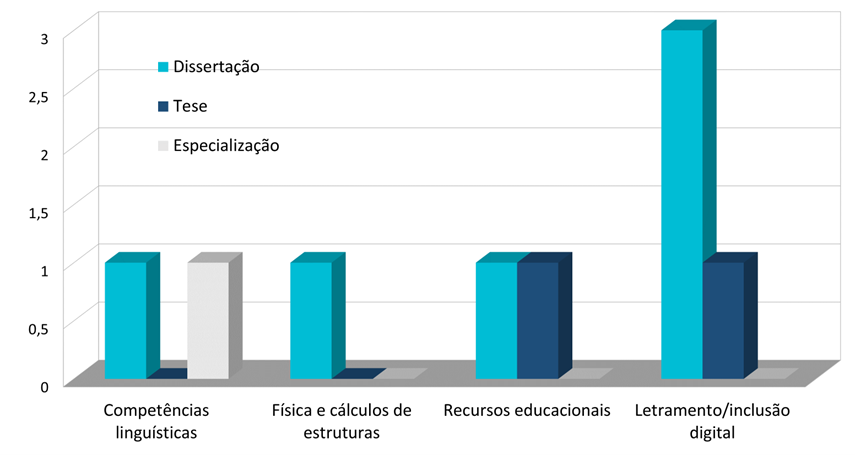
\includegraphics[width=\textwidth]{Fig7.png}
\source{as autoras.}
\end{minipage}
\end{figure}

Como pode-se verificar na \Cref{fig7}, a área de letramento e inclusão
digital se destacam com três dos outros trabalhos analisados. A tese de
\textcite[203~f.;~il.]{Tonelli2012} investigou como os estudantes do PROEJA fazem uso
das TDIC e os desafios de seu uso, visto que o mundo do trabalho requer
cada vez mais cidadãos com competências digitais. A dissertação de \textcite[60~f]{Lobo2012}, visa analisar as possibilidades da Educação a Distância (EaD)
como uma alternativa a Pedagogia da alternância, tendo como tema da
proposta EaD a inclusão digital. A autora aponta que o EaD tem muito a
contribuir com a pedagogia da alternância, ampliando os espaços e tempos
de aprendizagem.

\textcite{rocha_os_2019} aponta em seu trabalho que o letramento digital dos alunos
jovens e adultos está muito voltado a instrumentalidade das disciplinas
técnicas e pouco relacionado ao fortalecimento das questões
socioculturais, constituindo-se um desafio a formação integral dos
sujeitos. Este dado está dissonante da abordagem freiriana, que
possibilita compreender os aprendizes enquanto sujeitos históricos, como
citam \textcite{morais2023}.

A temática de competências linguísticas, apresenta dois trabalhos, sendo
que a dissertação de mestrado de \textcite{Santos2021} tinha como objetivo
avaliar como a ferramenta digital \emph{Storybord That} pode contribuir
para retextualização do gênero textual notícia e para ampliação do
universo de leitura de uma turma do PROEJA da Rede Federal de Ensino de
RO. Segundo o autor, o uso da ferramenta digital contribuiu para
retextualizar de um gênero para outro, preservando as informações do
texto base. O trabalho de conclusão de curso de especialização de
\textcite{Silveira2021} investiga como a prática da escrita em língua
estrangeira está inserida no contexto de um Curso de Agroindústria, na
modalidade PROEJA, bem como visa compreender como os estudantes veiculam
esta língua por meio das TDIC. A autora relata que as TDIC quando
planejadas e utilizadas de forma adequada, podem auxiliar o processo de
escrita.

O tema recursos educacionais para o PROEJA é abordado em uma tese e uma
dissertação. Na tese de \textcite[268f]{Bentes103}, o objeto de estudo é analisar
como os recursos educacionais digitais contribuem para prática
pedagógica no PROEJA. O autor apresenta a diferença do interesse do
público adulto, apontando limitações e dificuldades inerentes a
necessidade de letramento digital, o qual remete a temática acima
descrita. Por outro lado, a dissertação de \textcite{Souza2021} tem como foco a
produção de recursos educacionais digitais para uso na educação de
jovens e adultos do ensino profissionalizante. A autora relata a
importância de repositórios de objetos educacionais voltados para o
público do PROEJA, o que ficou evidente com as necessidades de aulas
digitais durante a pandemia do Covid-19.

O ensino de Física imbricado ao cálculo de estruturas foi o tema da
dissertação de \textcite[147~f.,~il]{Lima2022}, o qual explorou diferentes ferramentas,
dentre elas simulações da plataforma Phet\footnote{Plataforma digital de
	recursos educacionais Phet Colorado. Disponível em:
	\url{https://phet.colorado.edu/pt_BR/}}, visando uma aprendizagem
significativa. O autor aponta que a proposta de sequência didática se
mostrou viável, tendo contribuições significativas ao aprendizado dos
público-alvo.
